\section{Mô tả thiết kế phần mềm}
\subsection{Sơ đồ UML của phần mềm}
Do kích thước chiều ngang của giấy có hạn nên sơ đồ UML của phần mềm được đặt trong thư mục \textbf{UMLDiagram}, đính kèm với bản báo cáo này.

\subsection{Mô tả các lớp trong phần mềm}
\subsubsection{Lớp \lstinline{Settings}}
Lớp \lstinline{Settings} cung cấp một vài thông tin cài dặt cơ bản của game.\\
Sơ đồ UML của lớp \lstinline{Settings} như sau:

\begin{figure}[H]
\centering{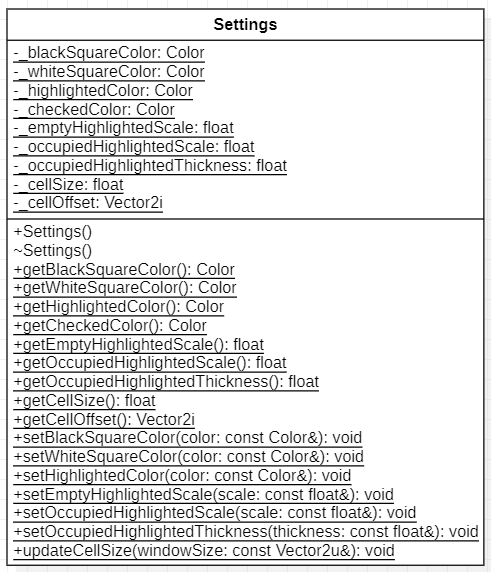
\includegraphics[scale=0.8]{images/classes/Settings}}
\caption{Sơ đồ UML của lớp \lstinline{Settings}}
\end{figure} 

Các thuộc tính (attributes) của lớp \lstinline{Settings} là thông tin về màu của các ô vuông trên bàn cờ, màu của ô vuông lúc được làm nổi bật (highlight), màu của ô vuông khi bị chiếu. Các màu này được dựa trên mã màu RGBA. Mã màu RGGA trong đồ án được lấy từ trang web: \url{https://rgbacolorpicker.com}. Ngoài ra, còn có các thuộc tính mô tả về tỉ lệ, độ dày mỏng của các nét highlight, cũng như kích thước và offset của ô vuông trên bàn cờ.\\
Các phương thức (methods) của lớp \lstinline{Settings} cung cấp các hàm getters và setters cho các thuộc tính của lớp.\\
Hầu hết các thuộc tính và phương thức của lớp \lstinline{Settings} (trừ hàm tạo $-$ constructor và hàm hủy $-$ destructor) đều được khai báo dưới dạng thuộc tính/phương thức tĩnh (\lstinline{method}), tạo ra sự tiện lợi khi ta cần gọi chúng, giúp ta không phải tạo một đối tượng mới mỗi khi muốn sử dụng đến các tính năng này.

\subsubsection{Các lớp enum}
\paragraph{Lớp enum \lstinline{GameSound}}
Lớp \lstinline{GameSound} cung cấp các loại âm thanh của game: âm thanh khi di chuyển quân cờ (MOVE), khi bắt quân (CAPTURE), khi chiếu (CHECK), khi chiếu hết (CHECKMATE) hay khi stalemate (trạng thái mà cả hai bên đều không còn nước nào có thể đi được).\\
Sơ đồ UML của lớp enum \lstinline{GameSound} như sau:
\begin{figure}[H]
\centering{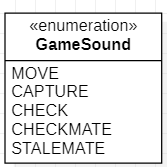
\includegraphics[scale=0.8]{images/classes/GameSound}}
\caption{Sơ đồ UML của lớp enum \lstinline{GameSound}}
\end{figure}

\paragraph{Lớp enum \lstinline{CellStatus}}
Lớp \lstinline{CellStatus} cung cấp các trạng thái của một ô vuông trên bàn cờ: đã có quân (OCCUPIED), chưa có quân (EMPTY) hay đang được highlight (HIGHLIGHTED).\\
Sơ đồ UML của lớp enum \lstinline{CellStatus} như sau:
\begin{figure}[H]
\centering{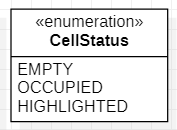
\includegraphics[scale=0.8]{images/classes/CellStatus}}
\caption{Sơ đồ UML của lớp enum \lstinline{CellStatus}}
\end{figure}

\paragraph{Lớp enum \lstinline{MoveType}}
Lớp \lstinline{MoveType} cung cấp thể loại của các nước di chuyển trong game: thăng cấp cho quân Tốt ($\mathrm{PROMOTION}$), nhập thành ngắn ($\mathrm{SHORT\_CASTLING}$), nhập thành dài ($\mathrm{LONG\_CASTLING}$), hoặc không phải các nước đi trên ($\mathrm{NONE}$).\\
Sơ đồ UML của lớp enum \lstinline{MoveType} như sau:
\begin{figure}[H]
\centering{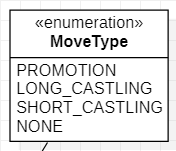
\includegraphics[scale=0.8]{images/classes/MoveType}}
\caption{Sơ đồ UML của lớp enum \lstinline{MoveType}}
\end{figure}

\paragraph{Lớp enum \lstinline{PieceType}}
Lớp \lstinline{PieceType} cung cấp các loại quân cờ: quân Vua (KING), quân Hậu (QUEEN), quân Tượng (BISHOP), quân Mã (KNIGHT), quân Xe (ROOK) và quân Tốt (PAWN).\\
Sơ đồ UML của lớp enum \lstinline{PieceType} như sau:
\begin{figure}[H]
\centering{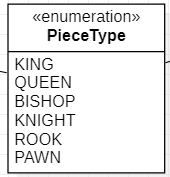
\includegraphics[scale=0.8]{images/classes/PieceType}}
\caption{Sơ đồ UML của lớp enum \lstinline{PieceType}}
\end{figure}

\paragraph{Lớp enum \lstinline{PieceDirection}}
Lớp \lstinline{PieceDirection} cung cấp hướng di chuyển thẳng về phía trước cho quân Tốt: đi lên (UP) đối với Tốt trắng và đi xuống (DOWN) đối với Tốt đen.\\
Sơ đồ UML của lớp enum \lstinline{PieceDirection} như sau:
\begin{figure}[H]
\centering{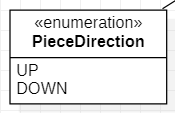
\includegraphics[scale=0.8]{images/classes/PieceDirection}}
\caption{Sơ đồ UML của lớp enum \lstinline{PieceDirection}}
\end{figure}

\paragraph{Lớp enum \lstinline{PieceColor}}
Lớp \lstinline{PieceColor} cho biết hai màu của người chơi/quân cờ: màu trắng (WHITE) và màu đen (BLACK).\\
Sơ đồ UML của lớp enum \lstinline{PieceColor} như sau:
\begin{figure}[H]
\centering{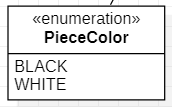
\includegraphics[scale=0.8]{images/classes/PieceColor}}
\caption{Sơ đồ UML của lớp enum \lstinline{PieceColor}}
\end{figure}

\subsubsection{Lớp \lstinline{ChessMove}}
Lớp \lstinline{ChessMove} cung cấp thông tin về nước đi trên bàn cờ.\\
Sơ đồ UML của lớp \lstinline{ChessMove} như sau:
\begin{figure}[H]
\centering{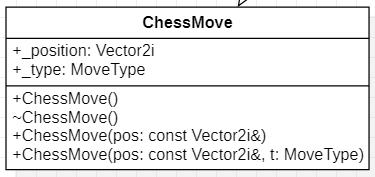
\includegraphics[scale=0.8]{images/classes/ChessMove}}
\caption{Sơ đồ UML của lớp enum \lstinline{ChessMove}}
\end{figure}
Các thuộc tính của lớp \lstinline{ChessMove} cho biết vị trí và thể loại của nước đi đó.\\
Các phương thức khởi tạo của lớp \lstinline{ChessMove} cho phép ta khởi tạo mặc định, khởi tạo với một tham số và khởi tạo với đầy đủ tham số.